% Critical strip, four partners of one zero, and a schematic zero-free boundary.
% sigma=0 at x=2.4, sigma=1/2 at x=3.7, sigma=1 at x=5.0.
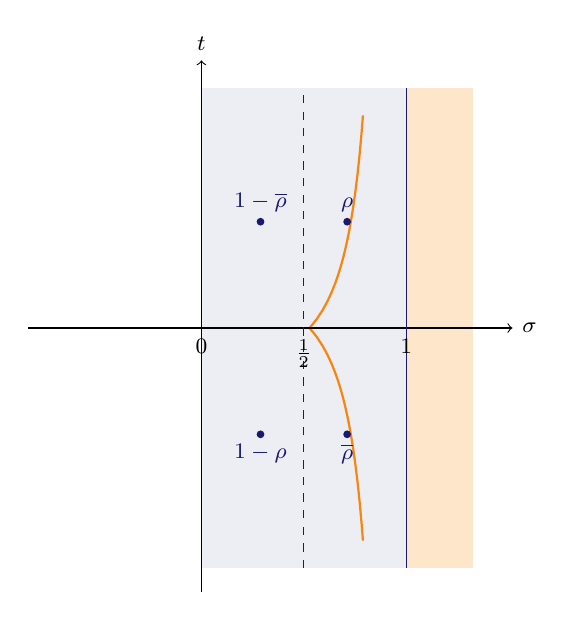
\begin{tikzpicture}[every node/.style={font=\footnotesize}]
  \fill[MidnightBlue!8] (2.4,-3.05) rectangle (5.0,3.05);
  \fill[BurntOrange!18] (5.0,-3.05) rectangle (5.85,3.05);
  \draw[BurntOrange,thick] plot[domain=-2.7:2.7,samples=49] ({5.0-0.85/ln(abs(\x)+2)},{\x});
  \draw[->] (0.2,0)--(6.35,0) node[right] {$\sigma$};
  \draw[->] (2.4,-3.35)--(2.4,3.4) node[above] {$t$};
  \draw[MidnightBlue,dashed] (3.7,-3.05)--(3.7,3.05);
  \draw[MidnightBlue] (5.0,-3.05)--(5.0,3.05);
  \node[below] at (2.4,-0.02) {$0$};
  \node[below] at (3.7,-0.02) {$\frac12$};
  \node[below] at (5.0,-0.02) {$1$};
  \fill[MidnightBlue] (4.25,1.35) circle (1.4pt) node[above] {$\rho$};
  \fill[MidnightBlue] (4.25,-1.35) circle (1.4pt) node[below] {$\overline{\rho}$};
  \fill[MidnightBlue] (3.15,1.35) circle (1.4pt) node[above] {$1-\overline{\rho}$};
  \fill[MidnightBlue] (3.15,-1.35) circle (1.4pt) node[below] {$1-\rho$};
\end{tikzpicture}
